%% Incluindo os pacotes necessários
\documentclass[12pt, a4paper]{article}
\usepackage[utf8]{inputenc}
\usepackage[portuguese]{babel}
\usepackage{booktabs}
\usepackage{titlesec}
\usepackage{titling}
\usepackage{enumitem}
\usepackage{indentfirst}
\usepackage{graphicx}
\graphicspath{{images/}}
\usepackage{fancyhdr}
\usepackage{color}
\usepackage{fancyhdr}
\usepackage{colortbl}
\usepackage{framed}

%% Definindo o Autor e o título
\author{Victor Emanuel Almeida \and Levi Cícero Arcanjo}
\title{Simulação e algorítimo de semáforos, para o problema ``Leitores e escritores''}

%% Estilo da página
\pagestyle{fancy}
\fancyhead[L]{}
\fancyhead[R]{}
\fancyfoot[L]{}
\fancyfoot[C]{}
\fancyfoot[R]{}
\renewcommand{\headrulewidth}{0.7pt}
\renewcommand{\footrulewidth}{0.3pt}

\titleformat{\section}
{\Large\bfseries}
{\thesection}
{.5cm}
{}[\titlerule]

\begin{document}
\maketitle\thispagestyle{fancy}

\section{Algorítimo}
\begin{figure}[!htb]
	\centering
	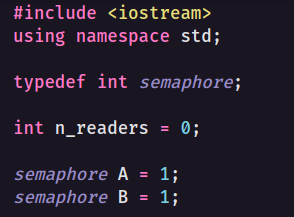
\includegraphics[keepaspectratio]{1.png}
	\caption{\label{fig:1.png}}
\end{figure}

\begin{figure}[!htb]
	\centering
	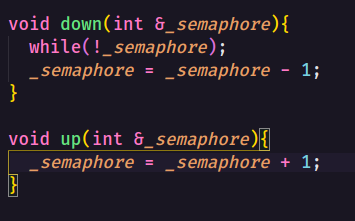
\includegraphics[keepaspectratio]{2.png}
	\caption{\label{fig:2.png}}
\end{figure}

\begin{figure}[!htb]
	\centering
	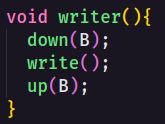
\includegraphics[keepaspectratio]{3.png}
	\caption{\label{fig:}}
\end{figure}

\begin{figure}[!htb]
	\centering
	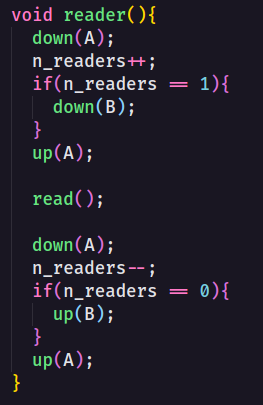
\includegraphics[keepaspectratio]{4.png}
	\caption{\label{fig:4.png}}
\end{figure}


\section{Simulação}
\begin{itemize}
	\item Tempo de criação:
	\begin{itemize}
			\item leitor 1 = momento 10
			\item leitor 2 = momento 4
			\item leitor 3 = momento 1
			\item escritor 1 = momento 14
			\item escritor 2 = momento 9
	\end{itemize}
	\item Tempo de execução:
		\begin{itemize}
			\item leitor 1 = momento 8
			\item leitor 2 = momento 7
			\item leitor 3 = momento 15
			\item escritor 1 = momento 6
			\item escritor 2 = momento 5
		\end{itemize}
\end{itemize}
	 
\begin{figure*}[!htb]
	\centering
	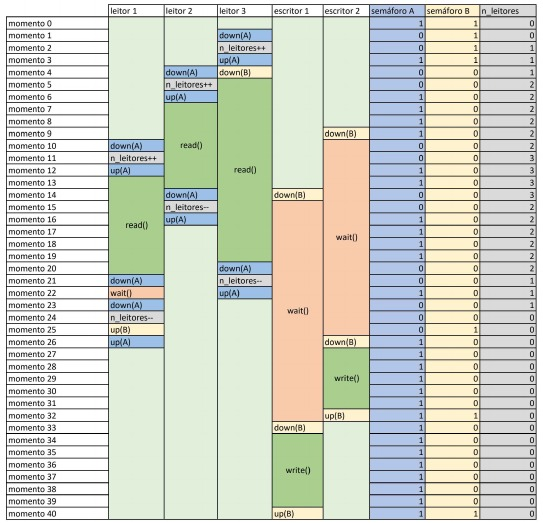
\includegraphics[keepaspectratio, width=\textwidth]{tabela.jpeg}
	\caption{\label{fig:tabela.pdf} Simulação do algorítimo}
\end{figure*}
\end{document}
